\documentclass{article}
\usepackage[utf8]{inputenc}
\usepackage[english]{babel}
\usepackage{geometry}
\geometry{a4paper, margin=0.9in}
\usepackage{pgfplots}
\usepackage{graphicx}
\usepackage{titlesec}


\title{Report on feature recognition {\&} face detection}
\author{Rafał Górniak \& Piotr Hynasiński}
\date{\today}

\begin{document}

\maketitle

\section{Custom CNN Model}
\subsection{Model Design and Architecture}
    The goal of this part of the project was to build and train a convolution neural network (CNN) model from scratch.
    As there are plenty of possibilities to do so, firstly we drew closer to subject area and ultimate purpose. Ordinary CNN consists of many layers, and each layer can consist of multiple layers. The most usual form of the model is input layer, hidden layer and output layer. The first one is simply input signal, in this case 2D, which is an image. Every neuron represents a pixel of the picture. The last layer is responsible for classification outcome, the returned data can be treated as a label possibility. Last, but not least the hidden layer, where computation and learning phase appear.

\vspace{0.2cm}
    In this paragraph, we will focus on the architecture, way of training, evaluation. The {\textit{GenderModel}}, which is CNN model capable of detecting being male or not, consists of four repeated cycles with {\textit{Convolution Layer}}, {\textit{Activation Function}}, and {\textit{Max Pooling}}. After getting input, data is redirected to {\textit{Con2d}}, torch convolution layer. As parameters there are: input channel number, which is 3 for RGB, output channel number, which is features/filter amount, each mask responsible for one particular feature, the kernel size, which is the mask size scanning the image. Then {\textit{ReLu}} reduces the number of pixels taken into account by resetting, so only the crucial ones, those with the biggest value leave. The function {\textit{MaxPool2d}} decrease dimensions by half. After four cycles of data processing, there are 128 frames with dimension 4x4.

    The output is transported to two {\textit{Fully Connected Layers}}, where the first flattens the set of matrices to 128, and the second one to 1. Between these two there is also dropout regularization function applied, which helps to prevent overfitting by randomly "dropping out" half of the neurons during training, thus stabilizing the learning process.

\subsection{Training Methodology}

    As model obtained dataset, the training phase can begin. Firstly, it is set into train mode and particular variables must be defined. These are: epochs number, early stop parameters: patience threshold, minimal difference. Even more important are loss functions and optimizer. The loss function used to measure how well the model's predictions match the ground truth during training and the optimization algorithm updates the model's weights based on the computed loss.
    We chose {\textit{BCEWithLogitsLoss}}, because it combines a sigmoid activation function and binary cross-entropy loss in a single operation, making it numerically stable and computationally efficient. On the other hand we have {\textit{Adam}}, probably the most commonly used gradient-based optimizer. It adjusts the learning rate for each parameter dynamically using moving averages of gradient. For its parameters we chose bolt 0.001, it ensures gradual learning to avoid overshooting the optimal solution.

\vspace{0.2cm}
    For each epoch, the gradients were minimized initially, ensuring that gradients from the previous batch do not interfere with the current batch. Then model performs a forward pass, producing predictions for output. The loss function computes the loss for the current batch, comparing actual labels with predicted ones. Then probably the most important part of the training phase is, back propagation with computing gradient loss. The last part is updating model's parameters using already computed values. Thanks to that, after each loop, model can evaluate validation set. If there is no progress, which means over fitting or wrong model adjustments, early stop breaks and finishes the training.

\subsection{Augmentation and loss-change}
    To increase model generalization and make it more uniform, certain augmentation transform was added. In ensures that not only nicely lightened and proper shaped with good people positioning images would be recognized properly, but also natural faces from common photographs. The measures are: vertical flip, random rotation with variation of 20 degrees, color jitter with slight brightness, contrast, saturation and hue change. It helped mainly to increase accuration in other sets, that the training was not based on, like {\textit{WIDER FACE}} and camera detection.

    In terms of balancing training model, we did check number of samples with different labels. It was pretty equal, and we decided that for amount of around ten thousands images in the input layer, it is not necessary to do so.

\vspace{0.2cm}
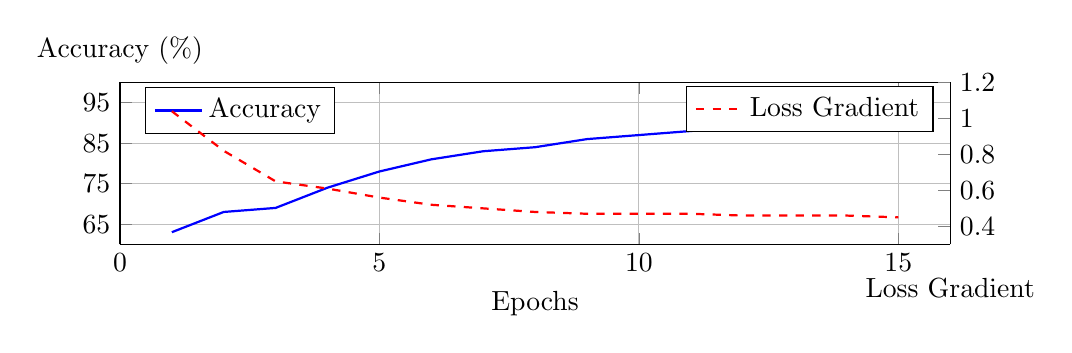
\begin{tikzpicture}
    \begin{axis}[
        width=\textwidth,
        height=0.3\textwidth,
        xlabel={Epochs},
        ylabel={Accuracy (\%)},
        y label style={yshift=-1em},
        xmin=0, xmax=16,
        ymin=60, ymax=100,
        xtick={0,5,10,15,20,25},
        ytick={65,75,85,95},
        legend pos=north west,
        grid=major,
        ymajorgrids=true,
        xmajorgrids=true,
        axis y line*=left,
        every axis y label/.style={at={(ticklabel* cs:1.05)}, anchor=south},
        ]

        % Accuracy data
        \addplot[blue, thick] coordinates {
            (1, 63) (2, 68) (3, 69) (4, 74) (5, 78)
            (6, 81) (7, 83) (8, 84) (9, 86) (10, 87)
            (11, 88) (12, 89) (13, 90) (14, 93) (15, 92)
        };

        \addlegendentry{Accuracy}
    \end{axis}

    \begin{axis}[
        width=\textwidth, % Match the width of the first axis
        height=0.3\textwidth,
        xlabel={Epochs},
        ylabel={Loss Gradient},
        y label style={yshift=-2em},
        axis y line*=right,
        axis x line=none,
        xmin=0, xmax=16,
        ymin=0.3, ymax=1.2,
        ytick={0.2,0.4,0.6,0.8,1.0,1.2},
        every axis y label/.style={at={(ticklabel* cs:-0.15)}, anchor=north},
        ]

        % Loss gradient data
        \addplot[red, thick, dashed] coordinates {
            (1, 1.04) (2, 0.82) (3, 0.65) (4, 0.61) (5, 0.56)
            (6, 0.52) (7, 0.50) (8, 0.48) (9, 0.47) (10, 0.47)
            (11, 0.47) (12, 0.46) (13, 0.46) (14, 0.46) (15, 0.45)
        };

        \addlegendentry{Loss Gradient}
    \end{axis}
\end{tikzpicture}

\begin{center}
\textbf{Graph 1.} Graph presenting change in accuracy performed on validation dataset and loss gradient on train dataset for gender detection. As it can be seen, they are bonded, inversely proportional to each other.
\end{center}

\vspace{0.2cm}
\section{Pre-trained CNN with  Fine-Tuning}

\subsection{Model Selection and Adaptation}
    There are loads of already trained model on much greater scale than that custom one in the first chapter. Having more diverse and better labeled set of images, such a model can recognize more complex and demanding patterns, not only for people, but everyday use utilities and stuff. We chose one of the {\textit{ResNet}} models, due to availability, simplicity of modifying and effectiveness.

    To customize the model after importing it, we made several adjustments to its structure. The most significant modification involved replacing the final fully connected layer, \textit{Linear}, to match the task requirements—in this case, adjusting the number of output neurons to one, as the model was designed to focus on detecting a "big nose" feature. Additionally, all layers except the last one were frozen to prevent changes to the weights and parameter values in the pre-trained layers. This ensured that only the newly added \textit{Linear} layer was trainable, allowing the model to specialize in the desired task without altering the pre-trained feature representations.

\subsection{Training Methodology}

For training, most of the parameters were the same as those used for the custom model. The learning rate was set to 1/1000
 , the optimizer used was Adam, and the loss function was binary cross-entropy. Additionally, early stopping was employed to prevent over-fitting, triggering after a maximum of three consecutive epochs with no improvement or worse accuracy.

One crucial aspect that was not mentioned previously is how the model's output was accessed and evaluated. The model's output was passed through a sigmoid function, which transformed the raw output into a probability value . If the resulting value was greater than 0.5, it was automatically considered as a positive class.

\subsection{Augmentation and loss-changes}
    Augmentation transformations conducted to increase model's capabilities are the same as for custom model. Fine Changes in angle, rotation, flip and color cause its advancement, not degrading as it could be with exaggeration.

\vspace{0.2cm}
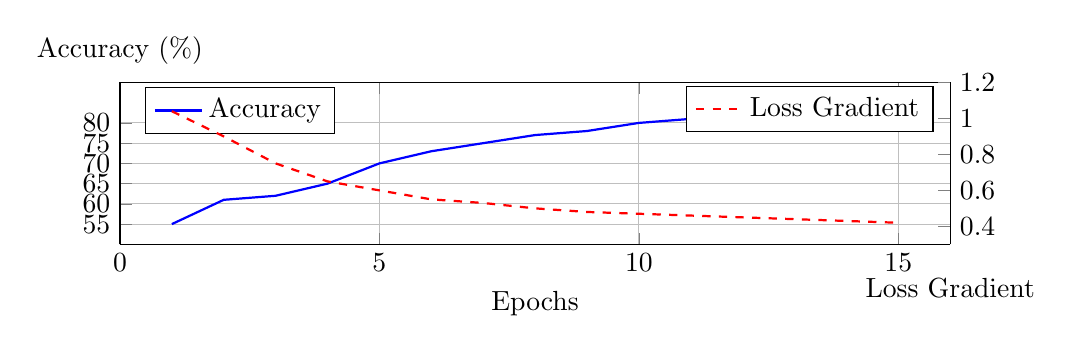
\begin{tikzpicture}
    \begin{axis}[
        width=\textwidth,
        height=0.3\textwidth,
        xlabel={Epochs},
        ylabel={Accuracy (\%)},
        y label style={yshift=-1em},
        xmin=0, xmax=16,
        ymin=50, ymax=90,
        xtick={0,5,10,15},
        ytick={55,60,65,70,75,80},
        legend pos=north west,
        grid=major,
        ymajorgrids=true,
        xmajorgrids=true,
        axis y line*=left,
        every axis y label/.style={at={(ticklabel* cs:1.05)}, anchor=south},
        ]

        % Accuracy data with rapid increase initially and then gradual improvement
        \addplot[blue, thick] coordinates {
            (1, 55) (2, 61) (3, 62) (4, 65) (5, 70)
            (6, 73) (7, 75) (8, 77) (9, 78) (10, 80)
            (11, 81) (12, 81) (13, 81) (14, 82) (15, 82)
        };

        \addlegendentry{Accuracy}
    \end{axis}

    \begin{axis}[
        width=\textwidth, % Match the width of the first axis
        height=0.3\textwidth,
        xlabel={Epochs},
        ylabel={Loss Gradient},
        y label style={yshift=-2em},
        axis y line*=right,
        axis x line=none,
        xmin=0, xmax=16,
        ymin=0.3, ymax=1.2,
        ytick={0.2,0.4,0.6,0.8,1.0,1.2},
        every axis y label/.style={at={(ticklabel* cs:-0.15)}, anchor=north},
        ]

        % Loss gradient data with occasional small adjustments
        \addplot[red, thick, dashed] coordinates {
            (1, 1.04) (2, 0.90) (3, 0.75) (4, 0.65) (5, 0.60)
            (6, 0.55) (7, 0.53) (8, 0.50) (9, 0.48) (10, 0.47)
            (11, 0.46) (12, 0.45) (13, 0.44) (14, 0.43) (15, 0.42)
        };

        \addlegendentry{Loss Gradient}
    \end{axis}
\end{tikzpicture}

\begin{center}
\textbf{Graph 2.} Graph showing the change in accuracy on the validation dataset and the loss gradient on the training dataset for big nose detection. Initially, the model quickly improves, but later, the progress becomes more gradual, with slight fluctuations at the end.
\end{center}
\vspace{0.2cm}
\section{Results on the CelebA Test Set}

After training and validating phase the custom CNN for gender classification and the fine-tuned ResNet for the “big nose” attribute, both models were evaluated on the CelebA test set. This dataset contains quite clean and varied portraits, allowing to examine performance of each model with the use of images with clear labels.

\subsection{CNN Model for Gender Classification}
On the CelebA test split, our custom CNN achieved high accuracy, mostly over 90\%. The confusion matrix for the gender classification task shows a lot of true positive and true negative results. It means that the model generally distinguished male and female faces effectively. Misclassifications were taking place in the case of images where lighting or hair made recognition of facial traits more challenging and less straightforward. The model was sometimes confused by angled poses. Nevertheless, the results show that the CNN was well-trained to handle well frontal faces.

\vspace{0.2cm}
\textbf\ Confusion matrix of CNN Model for Gender and Big-nose Classification
\begin{figure}[ht]
    \centering
    \begin{minipage}{0.3\linewidth}
        \centering
        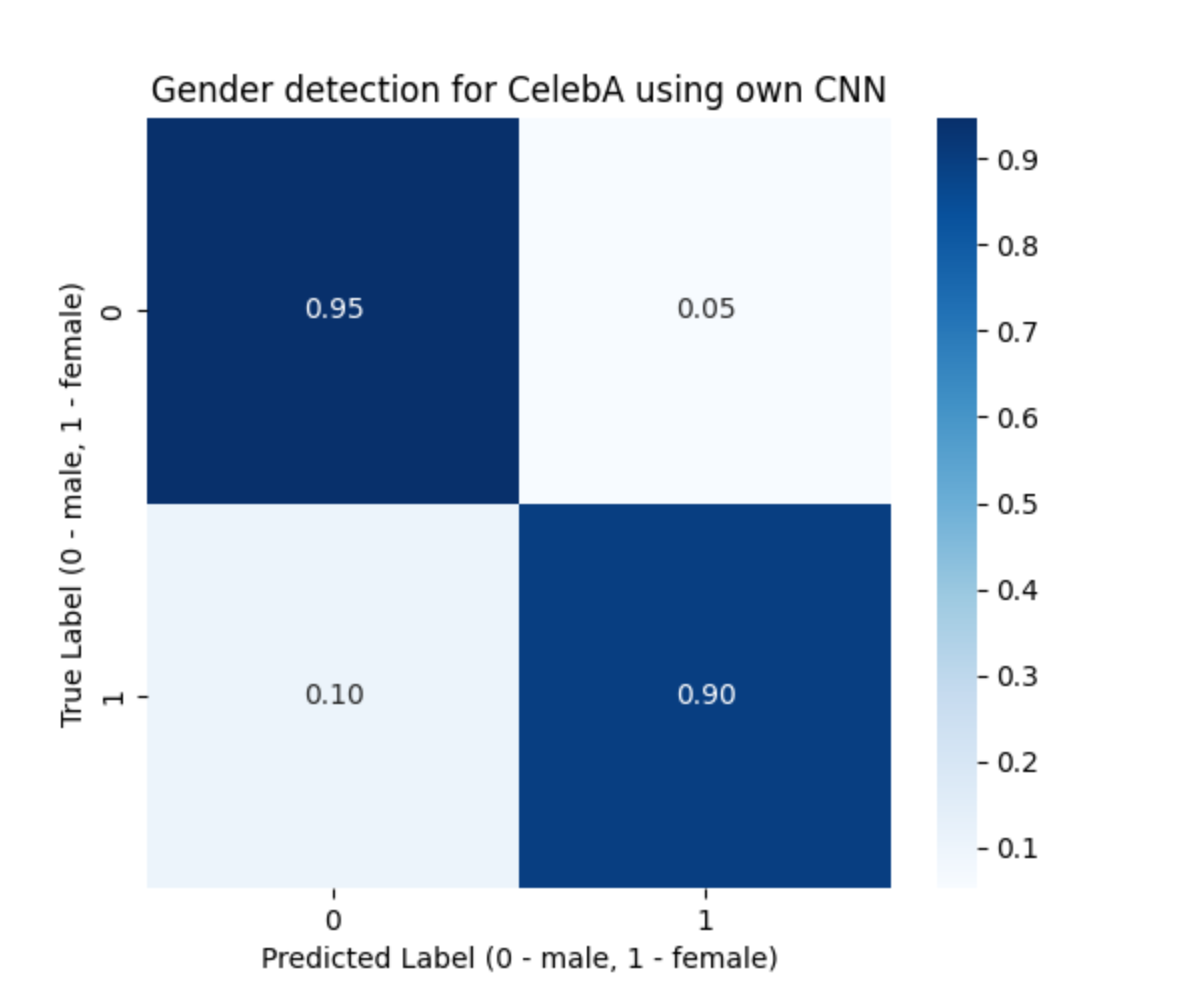
\includegraphics[width=\linewidth]{confusion_matrix_celeba_CNN.png}
        \caption{Gender with CNN}
        \label{fig:first}
    \end{minipage}
    \hspace{0.05\linewidth} s
    \begin{minipage}{0.3\linewidth}
        \centering
        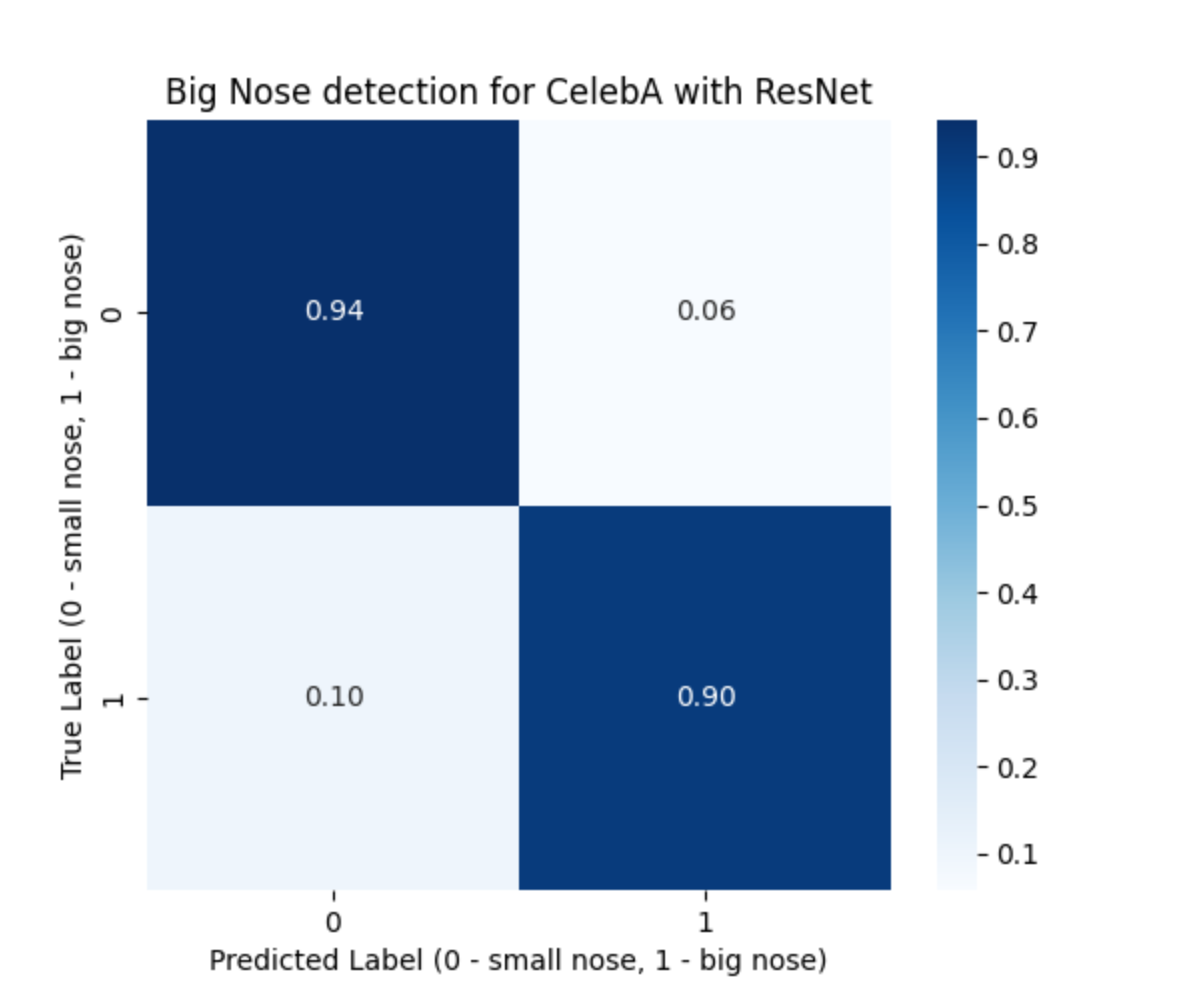
\includegraphics[width=\linewidth]{confusion_matrix_celeba_RESNET.png}
        \caption{Nose with ResNet}
        \label{fig:second}
    \end{minipage}
    \label{fig:side-by-side}
\end{figure}


\paragraph{Examples of Correct and Incorrect Classifications.}
In clear, frontal images with good lighting, the network correctly identified male and female faces. Misclassifications involved faces in bad lighting conditions, or faces that did not have clearly visible all facial features.
\vspace{0.2cm}
\begin{figure}[ht]
    \centering
    \begin{minipage}{0.2\linewidth}
        \centering
        \includegraphics[width=\linewidth]{000019.jpg}
        \label{fig:first}
    \end{minipage}
    \hspace{0.05\linewidth} s
    \begin{minipage}{0.2\linewidth}
        \centering
        \includegraphics[width=\linewidth]{image.png}
        \label{fig:second}
    \end{minipage}
    \label{fig:side-by-side}
\end{figure}


\subsection{ResNet Model for “Big Nose” Classification}
The ResNet model presented good performance, reaching around 90\% accuracy on CelebA for identifying whether a face had a “big nose” feature. The confusion matrix showed that the majority of faces were correctly classified. There were a few instances where noses were obscured by either some objects or bad lighting that caused problems with correct classification.

\vspace{0.2cm}
\textbf\ Confusion matrix of ResNet Model for Gender and Big-Nose Classification
\begin{figure}[ht]
    \centering
    \begin{minipage}{0.3\linewidth}
        \centering
        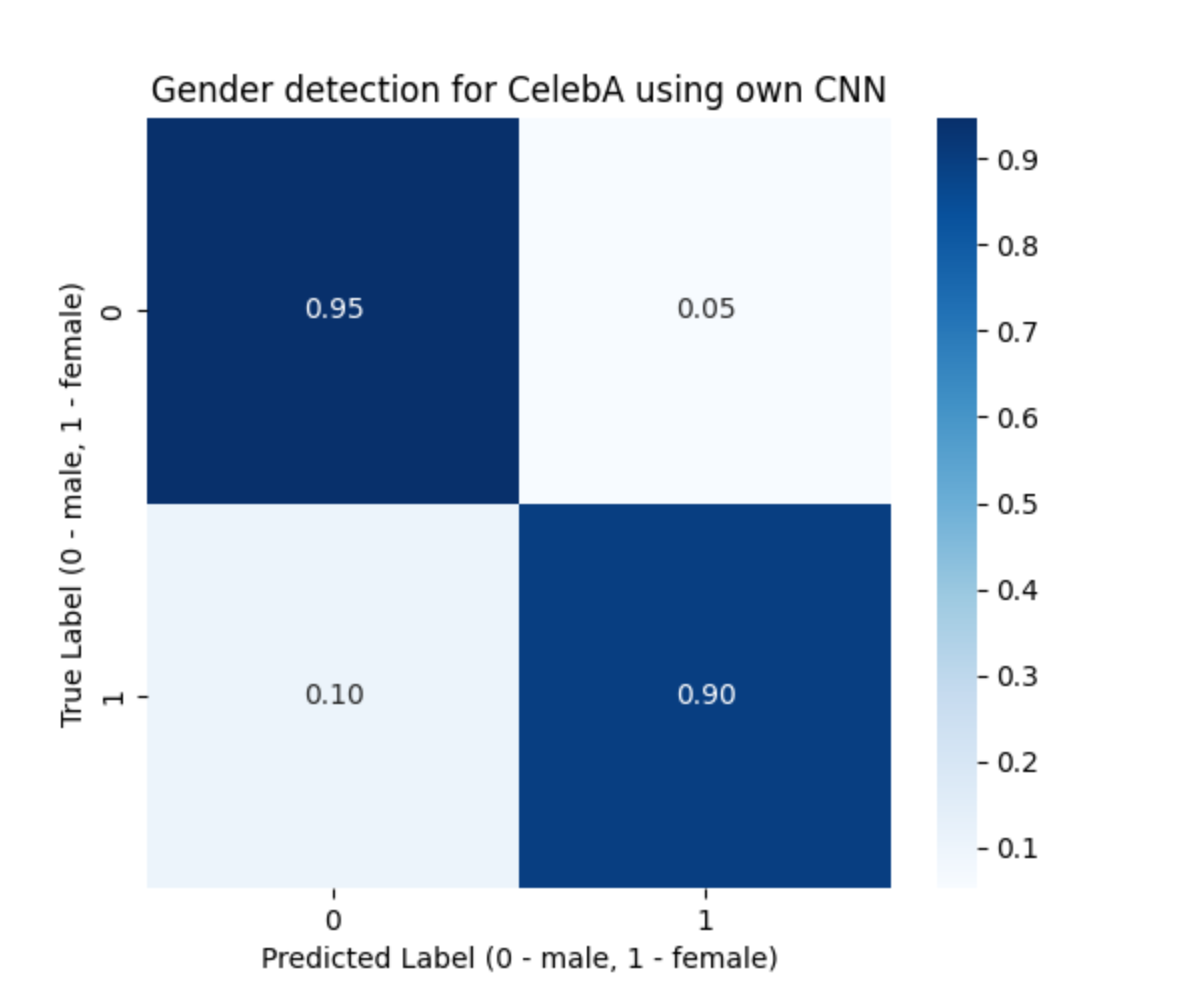
\includegraphics[width=\linewidth]{confusion_matrix_celeba_CNN.png}
        \caption{Gender with CNN}
        \label{fig:first}
    \end{minipage}
    \hspace{0.05\linewidth} s
    \begin{minipage}{0.3\linewidth}
        \centering
        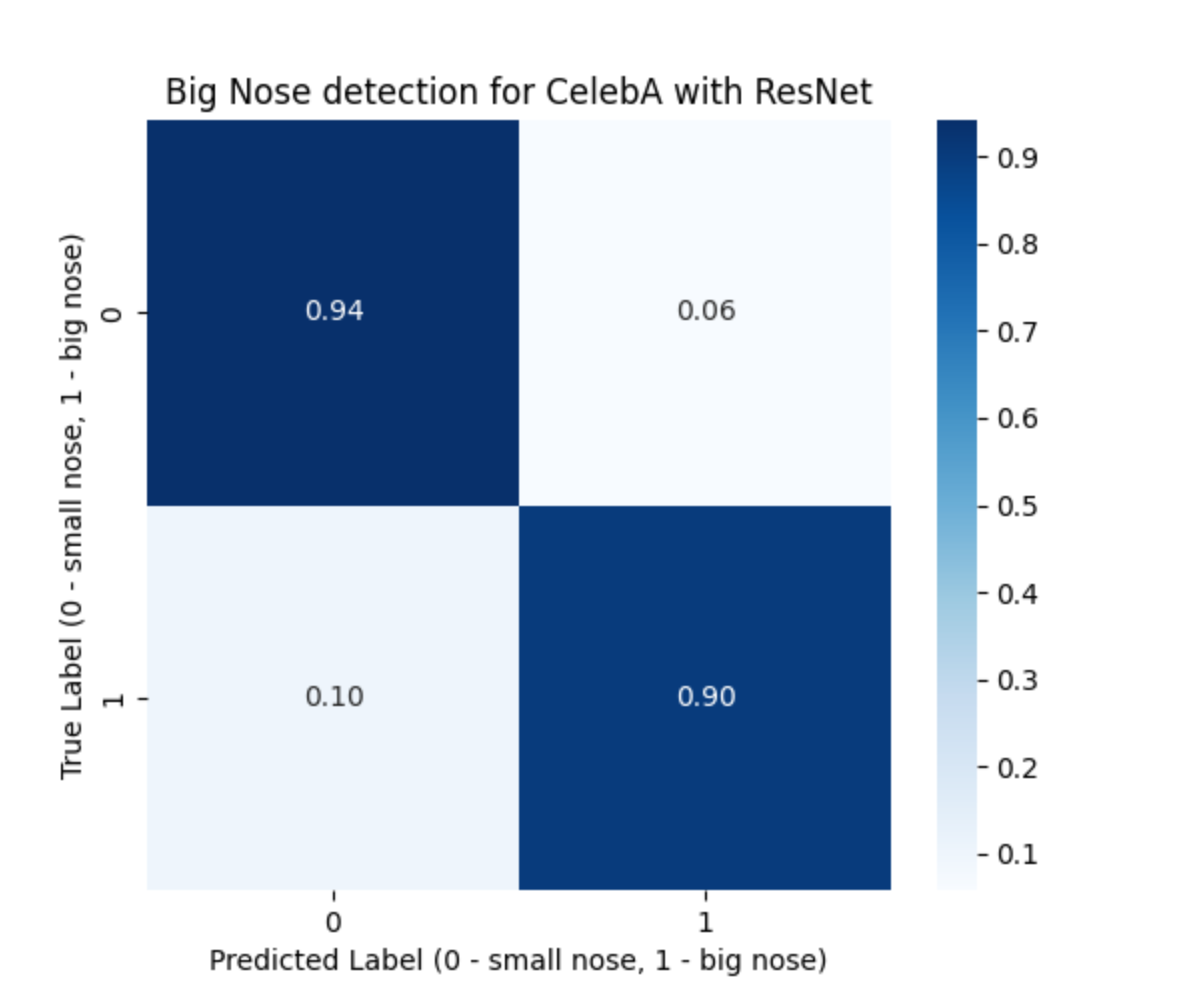
\includegraphics[width=\linewidth]{confusion_matrix_celeba_RESNET.png}
        \caption{Nose with ResNet}
        \label{fig:second}
    \end{minipage}
    \label{fig:side-by-side}
\end{figure}

\paragraph{Classification process}
There is no need to show another images of well and bad predicted photos. The outcomes are pretty much the same thanks to augmentation or image selection. Some are well interpreted, others not because of the same causes as mentioned in previous subsection.

\vspace{0.2cm}
\section{Results on the WIDERFace Dataset}

To assess the ability of models to handle more diverse and complex images, both the gender-classifying CNN and the “big nose” ResNet models were tested on a subset of the WIDERFace dataset. This subset comprised 100 images, each containing three to five faces. Since WIDERFace does not include the attributes needed, each face was manually annotated for gender and nose size.
The selected images exhibited non-frontal poses, a variety of lighting scenarios, and additional items like glasses, hats and more. Then, the preprocessing steps were applied to detected face regions as in the case of CelebA to maintain consistency.

\subsection{Gender Classification Results}
For gender classification, the custom CNN achieved roughly 86\% accuracy. It shows a small decline compared to the CelebA test set. Images where faces were significantly obscured by hats, masks, or other people decreased the accuracy. The confusion matrix proves that male faces were occasionally misclassified as female, and vice versa.

\subsection{“Big Nose” Classification Results}
For the “big nose” attribute, the ResNet experienced a comparable drop, achieving around 86\% accuracy. In some cases, moderate nose sizes were mistakenly identified as large, possibly due to shadows or other objects that intervened.

\subsection{Insights}
Although the data augmentation partially improved performance, the results suggest that adding more image examples of extreme poses, objects (hats, glasses), and low-light conditions could further improve generalization. Enhanced augmentation methods or fine-tuning on a dataset closer in style to WIDERFace might improve accuracy levels to match or exceed those on CelebA.

\section{Results in the Camera Test Program}

Both models were integrated into a real-time testing application. Using a webcam the program detected faces and then passed these cropped face images to our two trained models CNN for gender, and ResNet for nose.

\subsection{Test Setup and Observations}
Initial tests involved varied lighting conditions, background settings, and face orientations. Each detected face produced two predictions: a gender probability (male vs.\ female) and a “big nose” probability (above or below the 0.5 threshold). In everyday indoor lighting, with the camera relatively close to a frontal angle, the models performed similarly well to the CelebA tests.

\subsection{Examples of Correct Detection}
Under moderately controlled conditions such as sufficient light, a clear view of the face, and minimal obstructions both models reliably classified gender and nose size in real time. Even slight head tilt or light intensity did not drastically reduce accuracy.

\begin{figure}[ht]
    \centering
    \begin{minipage}{0.45\linewidth}
        \centering
        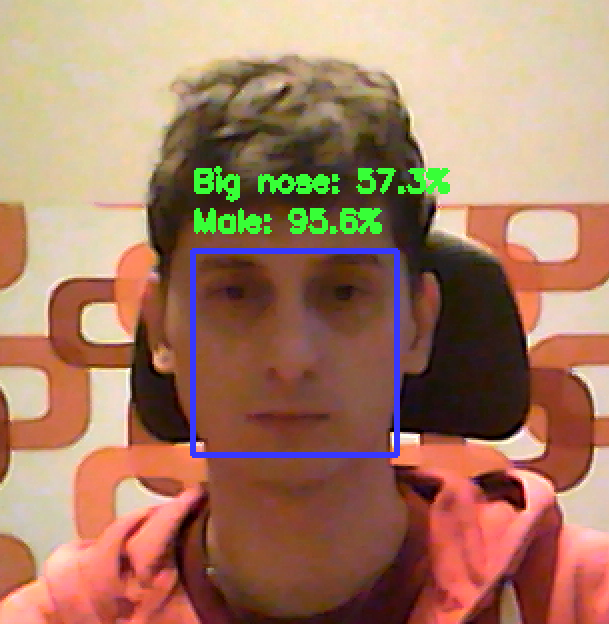
\includegraphics[width=\linewidth]{faceTest_camera_1.png}
        \caption{Sample image}
        \label{fig:first}
    \end{minipage}
    \hfill
    \begin{minipage}{0.45\linewidth}
        \centering
        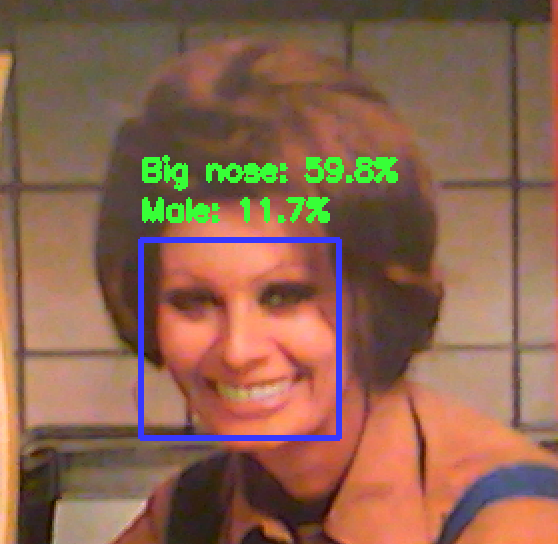
\includegraphics[width=\linewidth]{faceTest_camera_2.png}
        \caption{Sample image}
        \label{fig:first}
    \end{minipage}
    \label{fig:side-by-side}
\end{figure}

\subsection{Challenges and Limitations}
In brightly backlit scenes or with unusual camera angles the models made more mistakes. It matches the previous observations.

\subsection{Conclusions on Camera Testing}
Despite the challenges, the camera test program demonstrated that models are capable of near real-time inference and can maintain a decent level of accuracy in everyday environments. Overall, the conclusions from this test are similar to the ones from the previous tests: with sufficient data augmentation and robust architectures, the models generalize quite well the real-world scenarios.


\end{document}